%%%%%%%%%%%%%%%%%%%%%%%%%%%%%%%%%%%%%%%%%%%%%%%%%%%%%%%%%%%%%%%%%%%%%%%%%%%%%%%%%%%%%%%%%%%%%%%%%%%%%%%
%%%%%%%%%%%%%% Template de Artigo Adaptado para Trabalho de Diplomação do ICEI %%%%%%%%%%%%%%%%%%%%%%%%
%% codificação UTF-8 - Abntex - Latex -  							     %%
%% Autor:    Fábio Leandro Rodrigues Cordeiro  (fabioleandro@pucminas.br)                            %% 
%% Co-autores: Prof. João Paulo Domingos Silva, Harison da Silva e Anderson Carvalho		     %%
%% Revisores normas NBR (Padrão PUC Minas): Helenice Rego Cunha e Prof. Theldo Cruz                  %%
%% Versão: 1.1     18 de dezembro 2015                     %%
%%%%%%%%%%%%%%%%%%%%%%%%%%%%%%%%%%%%%%%%%%%%%%%%%%%%%%%%%%%%%%%%%%%%%%%%%%%%%%%%%%%%%%%%%%%%%%%%%%%%%%%
\section{Alfabeto $\Sigma$} 
\begin{itemize}
\item final
\item else
\item (
\item <=
\item ;
\item write
\item int
\item \&\&
\item )
\item ,
\item begin
\item writeln
\item byte
\item ||
\item <
\item +
\item endwhile
\item TRUE
\item string
\item !
\item >
\item -
\item endif
\item FALSE
\item while
\item <-
\item !=
\item *
\item endelse
\item boolean
\item if
\item =
\item >=
\item /
\item readln 
\end{itemize}

\section{\esp Lexemas e Padrão de formação}
\begin{table}[!h]
\centering
\caption{Lexema x Padrão de formação}
\vspace{0.2cm}
\begin{tabular}{r|lr}
 
Posi{\c c}{\~a}o & Lexema & Padr{\~a}o de Forma{\c c}{\~a}o \\ % Note a separação de col. e a quebra de linhas
\hline                               % para uma linha horizontal
1 & final & (f\cup F)(i\cup I)(n\cup N)(a\cup A)(l\cup L) \\
2 & else & (e\cup E)(l\cup L)(s\cup S)(e\cup E) \\
3 & ( & ( \\
4 & <= & <= \\
5 & ; & ; \\
6 & write & (w\cup W)(r\cup R)(i\cup I)(t\cup T)(e\cup E) \\
7 & int & (i\cup I)(n\cup N)(t\cup T) \\
8 & \&\& & \&\& \\
9 & ) & ) \\
10 & , & , \\
11 & begin & (b\cup B)(e\cup E)(g\cup G)(i\cup I)(n\cup N) \\
12 & writeln & (w\cup W)(r\cup R)(i\cup I)(t\cup T)(e\cup E)(l\cup L)(n\cup N) \\
13 & byte & (b\cup B)(y\cup Y)(t\cup T)(e\cup E) \\
14 & || & || \\
15 & < & < \\
16 & + & + \\
17 & endwhile & (e\cup E)(n\cup N)(d\cup D)(w\cup W)(h\cup H)(i\cup I)(l\cup L)(e\cup E) \\
18 & TRUE & TRUE \\
19 & string & (s\cup S)(t\cup T)(r\cup R)(i\cup I)(n\cup N)(g\cup G) \\
20 & ! & ! \\
21 & > & > \\
22 & - & - \\
23 & endif & (e\cup E)(n\cup N)(d\cup D)(i\cup I)(F\cup f) \\
24 & FALSE & FALSE \\
25 & while & (w\cup W)(h\cup H)(i\cup I)(l\cup L)(e\cup E) \\
26 & <- & <- \\
27 & != & !=  \\
28 & * & * \\
29 & endelse & (e\cup E)(n\cup N)(d\cup D)(e\cup  E)(l\cup L)(s\cup S)(e\cup E) \\
30 & boolean & (b\cup B)(o\cup O)(o\cup O)(l\cup L)(e\cup E)(a\cup A)(n\cup N) \\
31 & if & (i\cup I)(F\cup f) \\
32 & = & = \\
33 & >= & >= \\
34 & / & / \\
35 & readln & (r\cup R)(e\cup E)(a\cup A)(d\cup  D)(l\cup L)(n\cup N) \\
\end{tabular}
\end{table}

    


\section{\esp Analisador Léxico - AFD}
\begin{center}    
\begin{figure}[!ht]
	\vspace{0.2cm}
	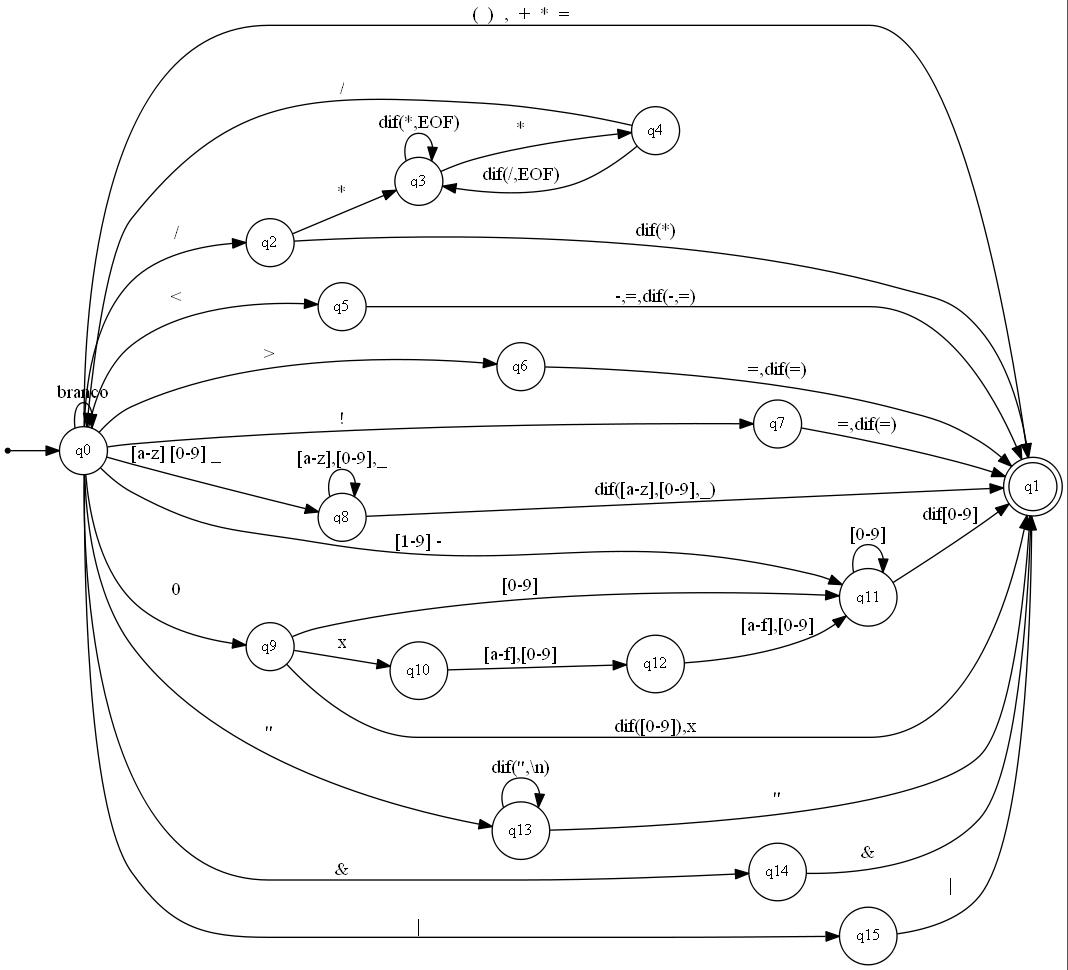
\includegraphics[width=0.9\textwidth]{figuras/automato.jpg}
	% Caption centralizada
	% Caption e fonte 
	 \vspace{0.2cm}
	\label{fig:figura1}
\end{figure}
\vspace{0.2cm}
\end{center}


\section{\esp Gramática com Expressões Regulares - GER}
\begin{center}    
\begin{figure}[!ht]
	\vspace{0.2cm}
	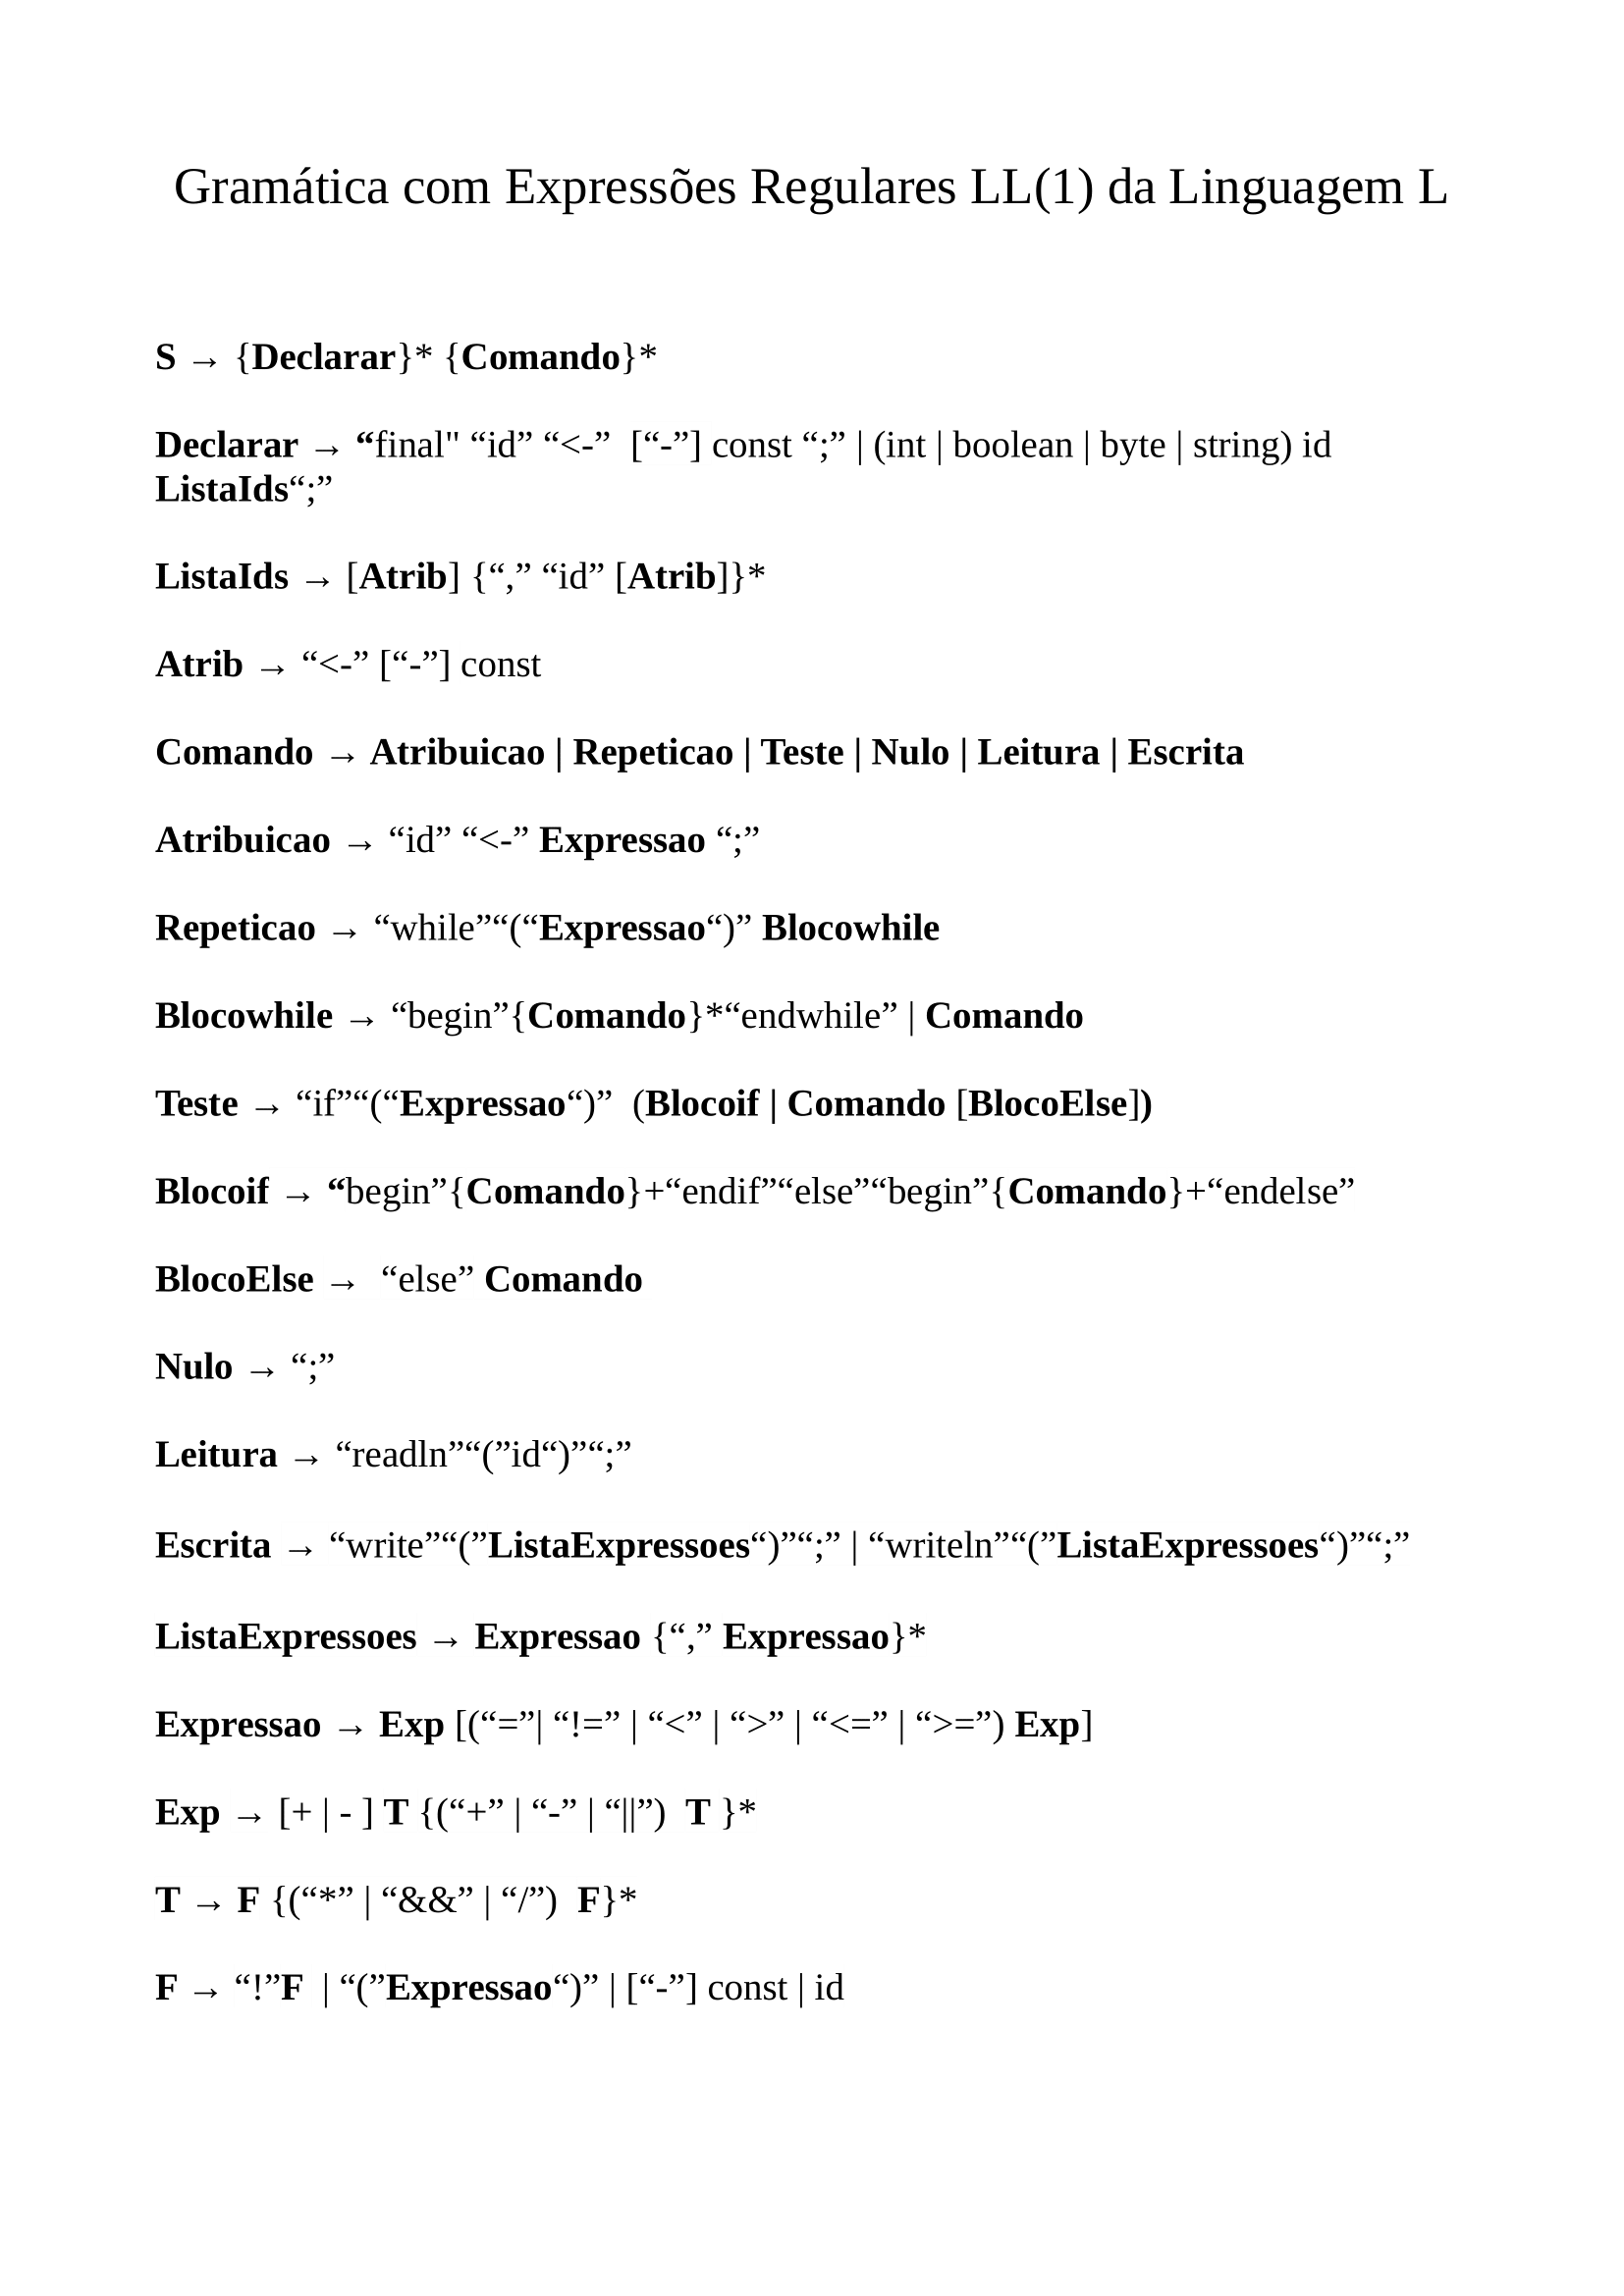
\includegraphics[width=0.9\textwidth]{figuras/GER_LL1-1.png}
	% Caption centralizada
	% Caption e fonte 
	 \vspace{0.2cm}
	\label{fig:figura1}
\end{figure}
\vspace{0.2cm}
\end{center}
% \subsection{\esp Trabalhos futuros}
% 
% Sugestões de estudos posteriores são ser adicionados subseção deste capítulo de conclusão.
